%---Objects ---------------------------------------------------
\begin{frame}[fragile] \frametitle{Objects}
\begin{itemize}
  \item an object is a dictionary: string $\rightarrow$ any value
  \item objects have properties - a (string, value) par in the dictionary (attributes, methods)
  \item properties can have any name, including reserved words and operations
  \item access properties using:
  \begin{itemize}
    \item dot notation: \code{myObj.prop}
    \item array index notation: \code{myObj['prop']}
  \end{itemize}
  \item properties are not in scope of methods, must use \code{this}
  \item \code{typeof objRef === 'object'}
  \item add properties by writing to them \code{myObj.newProp = 'adding stuff';}
  \item remove properties by: \code{delete myObj.newProp}
\end{itemize}
\end{frame}

%--- Create Objects ---------------------------------------------------
\begin{frame}[fragile] \frametitle{Create Objects}
\begin{itemize}
  \item object literals $\{prop: value\}$
  \item \code{new ConstructorFunction(args);}
\end{itemize}
\end{frame}

%---Object Literals ---------------------------------------------------
\begin{frame}[fragile] \frametitle{Object Literals}
\begin{itemize}
  \item superset of JSON
  \item comma separated list of properties inside \code{\{ \}}
  \item a property is defined by:
  \begin{itemize}
    \item \code{property-name : value}
    \item \code{method(parameters) \{ statements \}}
  \end{itemize}
  \item name in plain text, quotes if needed 
  \item value is any JavaScript expression
  \item \code{\{a:a\}} is the same as \code{\{a\}}
\end{itemize}
\end{frame}

%---Object Literals ---------------------------------------------------
\begin{frame}[fragile] \frametitle{Object Literals}
\begin{CodeBox}{object literal}
const familyName = 'Andersson';
const myObject = {
  givenName: 'Per',
  familyName,
  selector: 'givenName',
  getValue: function () {
    return this[this.selector];
  },
  setValue(value) {
    this[this.selector] = value;
  },
  '+': 'plus'
 }
\end{CodeBox}
\end{frame}

%---Object Literals 2 ---------------------------------------------------
\begin{frame}[fragile] \frametitle{Object Literals}
\begin{itemize}
  \item object literals are cheap
  \item use them frequently
  \item they bring structure and readability to programs
\end{itemize}
\begin{CodeBox}{object literals}
let myPoints = [{x: 0, y: 0}, {x:10, y:15}];

function foo(x, y, a, b, c, d) {
 console.log('b = '+ b);
}
function bar(x, y, options) {
 console.log('b = '+ options?.b);
}
\end{CodeBox}
\end{frame}

%--- Named Parameters ---------------------------------------------------
\begin{frame}[fragile] \frametitle{Named Parameters}
Remember, \code{foo} and \code{bar} prints option \code{b}.
\vspace{5mm}
\begin{CodeBox}{What is printed?}
foo(0, 0, 0, 0, 1, undefined, 1);
bar(0, 0, {a: 0, b: 1, d:1});
\end{CodeBox}
\vspace{10mm}
Did you notice thet foo have one extra parameter compared to the arguments list?
\\ Too few, or extra parameters do not raise errors in JavaScript. 
\end{frame}

%--- Constructor Functions ---------------------------------------------------
\begin{frame}[fragile] \frametitle{Constructor Functions}

\begin{itemize}
  \item same purpose as classes in Java
  \begin{itemize}
    \item initialises objects when used with \code{new}
  \end{itemize}
  \item are	 function, intended use differs
  \begin{itemize}
    \item \code{function ConstructorFunction(args) \{ ... \}}
    \item by convention: use leading capital letter
  \end{itemize}
  \item \code{new ConstructorFunction(args)} will:
  \begin{enumerate}
    \item creates an empty object
    \item set up inheritance
    \item calls \code{ConstructorFunction(args)} with the new object as \code{this}
    \item the constructor function adds properties to \code{this} and assign them values
    \item the result of \code{new} is the value returned by the \emph{constructor function}\\
             remember: the default return value of functions called by \code{new} is \code{this}
  \end{enumerate}
\end{itemize}
\end{frame}

%--- Constructor Functions  Example ---------------------------------------------------
\begin{frame}[fragile] \frametitle{Constructor Function Example}

\begin{columns}[onlytextwidth]
  \begin{column}{0.5\textwidth}
\begin{CodeBox}{class definition}
function Point(x, y) {
  this.x = x || 0;
  this.y = y || 0;
  this.getX = function() {
    return this.x;
  }
}
\end{CodeBox}
  \end{column}
  \begin{column}{0.5\textwidth}
\begin{CodeBox}{create instances}
let point1 = new Point(3, 6);
let point2 = new Point();
let point2 = new Point(5);
let point3 = 
  new Point(undefined, 5);
\end{CodeBox}
  \end{column}
\end{columns}%
\end{frame}

%--- this---------------------------------------------------
\begin{frame}[fragile] \frametitle{this}
\begin{itemize}
  \item \code{this} is defined in all functions
  \item its value depends on how the function is called:
  \begin{itemize}
    \item function call: \code{foo()} - the global object
    \item dot notation: \code{obj.foo()} - the object left of the dot
    \item explicit: \code{Function.prototype.call()}
    \item explicit: \code{Function.prototype.bind()} - creates a new function with a predefined value for \code{this}
    \item as an DOM event handler - the element the event fired from (not all cases for all browsers)
    \item as an inline DOM event handler - the DOM element on which the listener is placed
  \end{itemize}
  \item arrow functions: \code{this} from the enclosing scope is used
\end{itemize}
\end{frame}

%--- self---------------------------------------------------
\begin{frame}[fragile] \frametitle{self}
When a function is a ``object method''
\begin{itemize}
  \item you do not know if \code{this} refers to the right object
  \item use closure to fix this
  \item or use arrow functions
\end{itemize}
\begin{CodeBox}{}
function Person() {
  const self = this; // Some choose `that` instead of `self`. 
                           // Choose one and be consistent.
  self.age = 0;
  this.birthday = function() { self.age++; };
  this.birthday2 = _ =>  this.age++;
}
let per = new Person();
setInterval(per.birthday, 1000);
\end{CodeBox}
\end{frame}

%--- Prototype based Inheritance ---------------------------------------------------
\begin{frame}[fragile] \frametitle{Prototype Based Inheritance}

\begin{itemize}
  \item all object inherit from another object or \code{null}
  \item default is \code{Object}
  \item objects forms a \emph{prototype chain}
  \item property name lookup follows the prototype chain
  \item the chain ends with \code{null}
  \item you can access the prototype chain (but don't):
  \begin{itemize}
    \item \code{Object.getPrototypeOf(object)}
    \item \code{Object.setPrototypeOf(object, chain)}
  \end{itemize}
\end{itemize}
\end{frame}

%---------------------------------------------------------------------------------
\begin{frame}[fragile]
\frametitle{Prototype Chain}
  \centering
  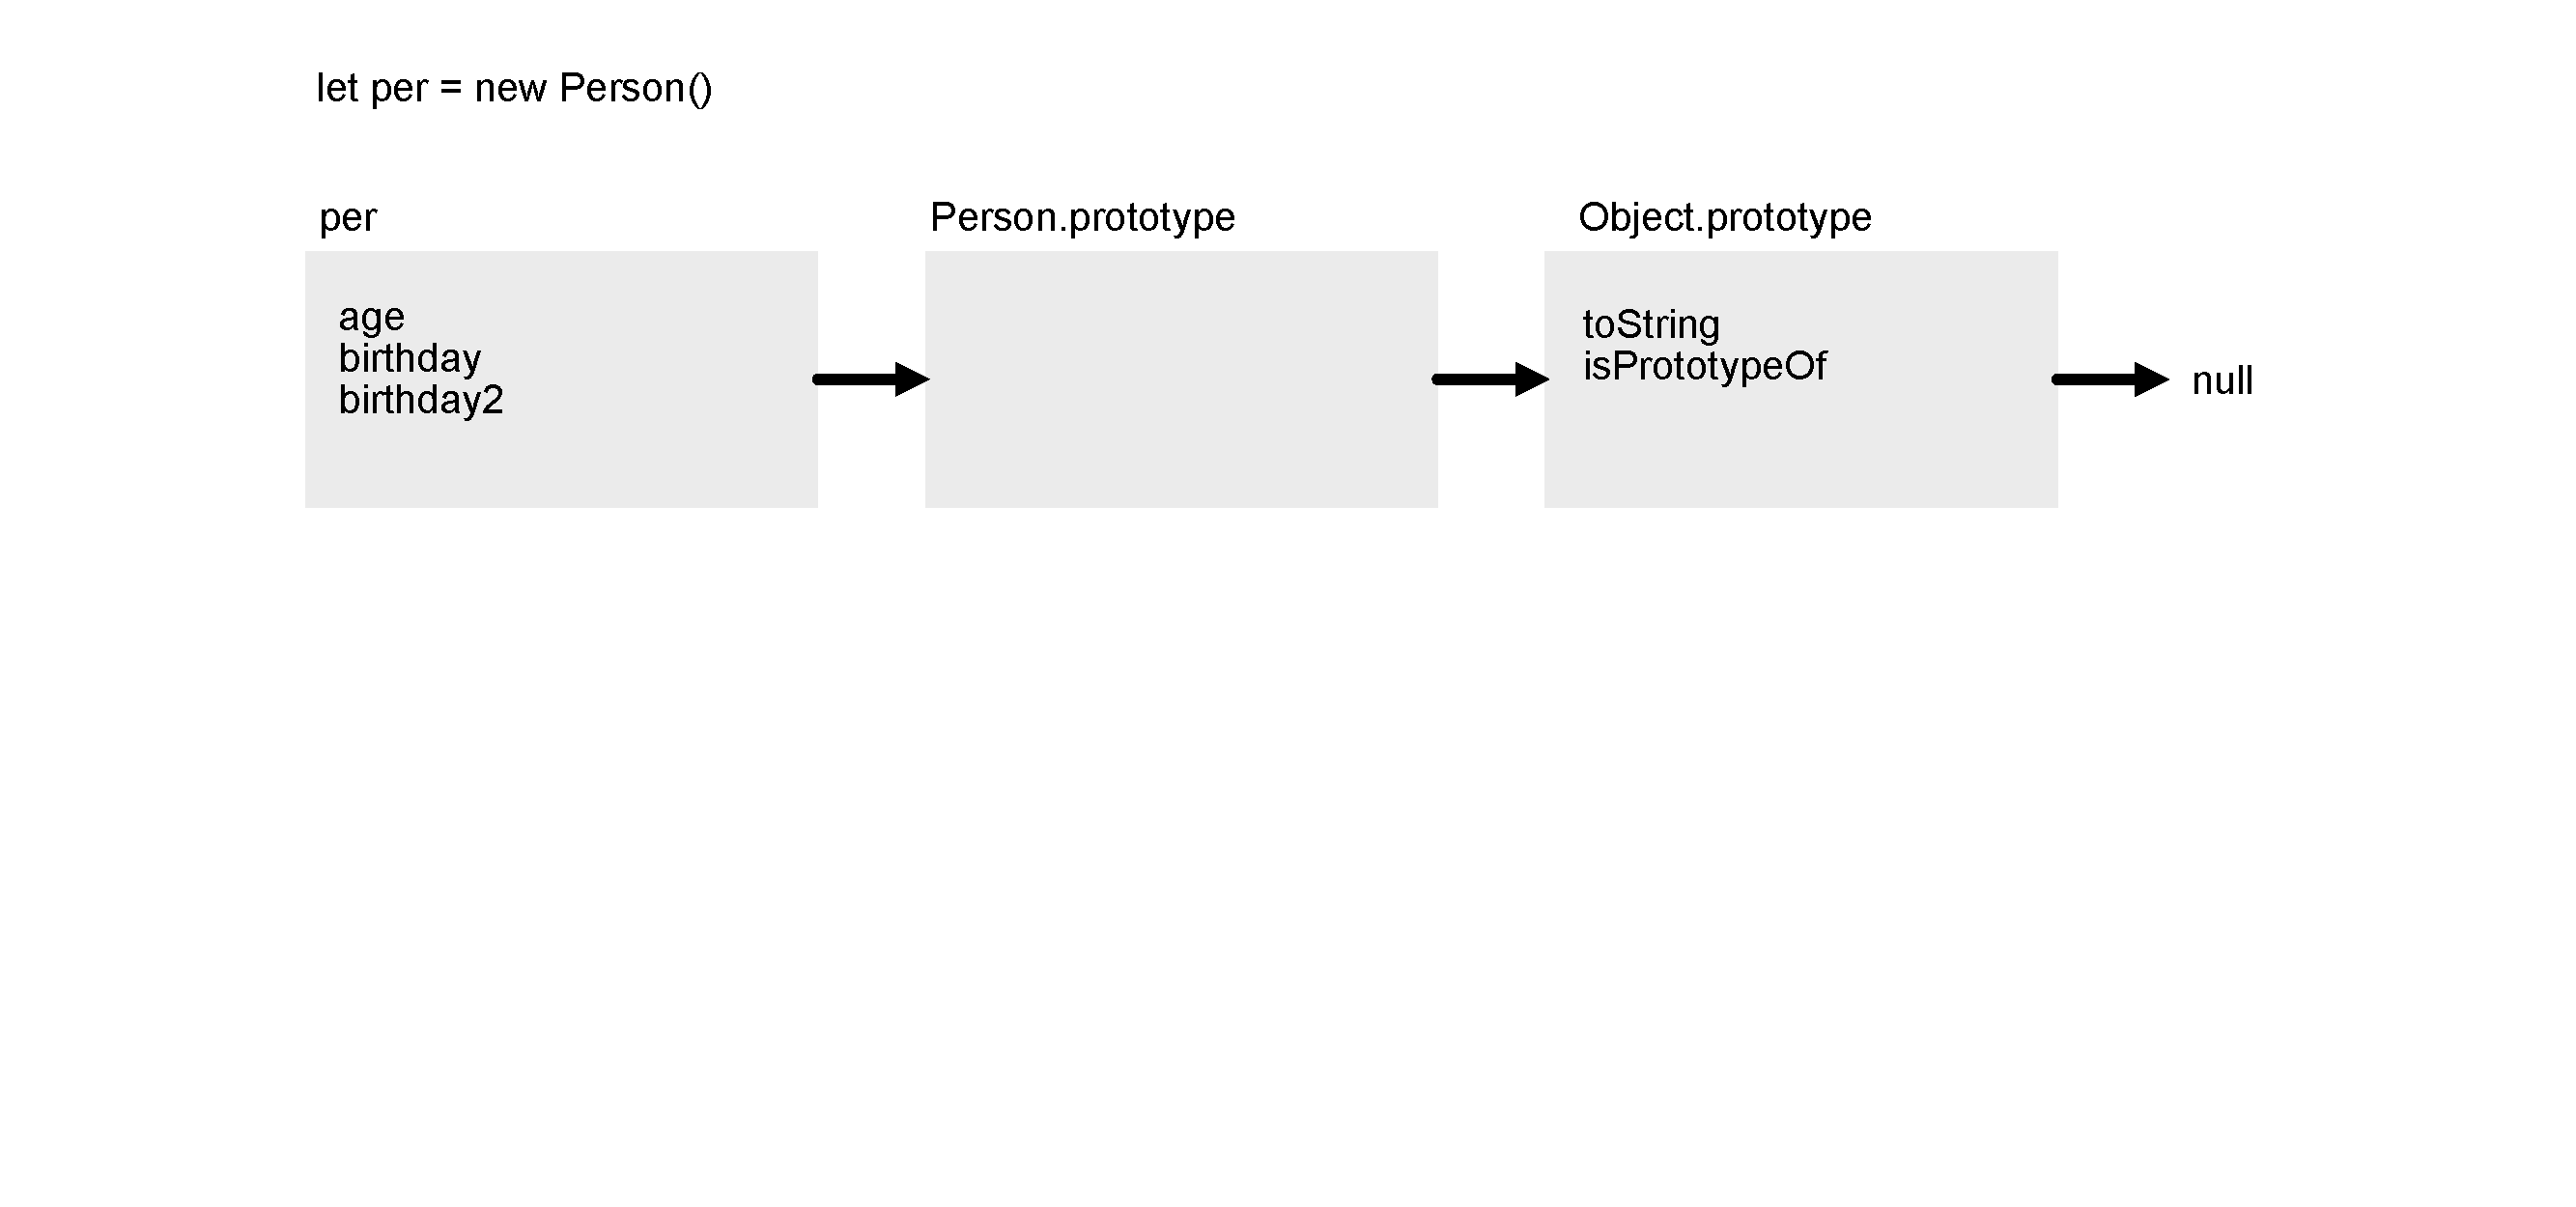
\includegraphics[width=14cm]{img/prototype_chain}

\end{frame}

%--- Function Object ---------------------------------------------------
\begin{frame}[fragile] \frametitle{Function Object}
Every functions is stored in a function object:
\begin{itemize}
  \item Function object:
  \begin{itemize}
    \item stores the function body
    \item the value of function expression: \code{function()\{  \}}
    \item is callable, left hand side of ()
    \item store static properties
    \item inherits from \code{Function.prototype}
    \item constructor functions must have the property \code{prototype}
      \begin{itemize}
      \item all functions except: methods, arrow functions, or async functions
      \end{itemize}
  \end{itemize}
\end{itemize}
\begin{itemize}
  \item Prototype object:
  \begin{itemize}
    \item added to the \emph{prototype chain} by \code{new}
    \item store inherited properties
    \item \code{constructor} refers to the function object
  \end{itemize}
\end{itemize}
\end{frame}

%---------------------------------------------------------------------------------
\begin{frame}[fragile]
\frametitle{Prototype Chain}
  \centering
  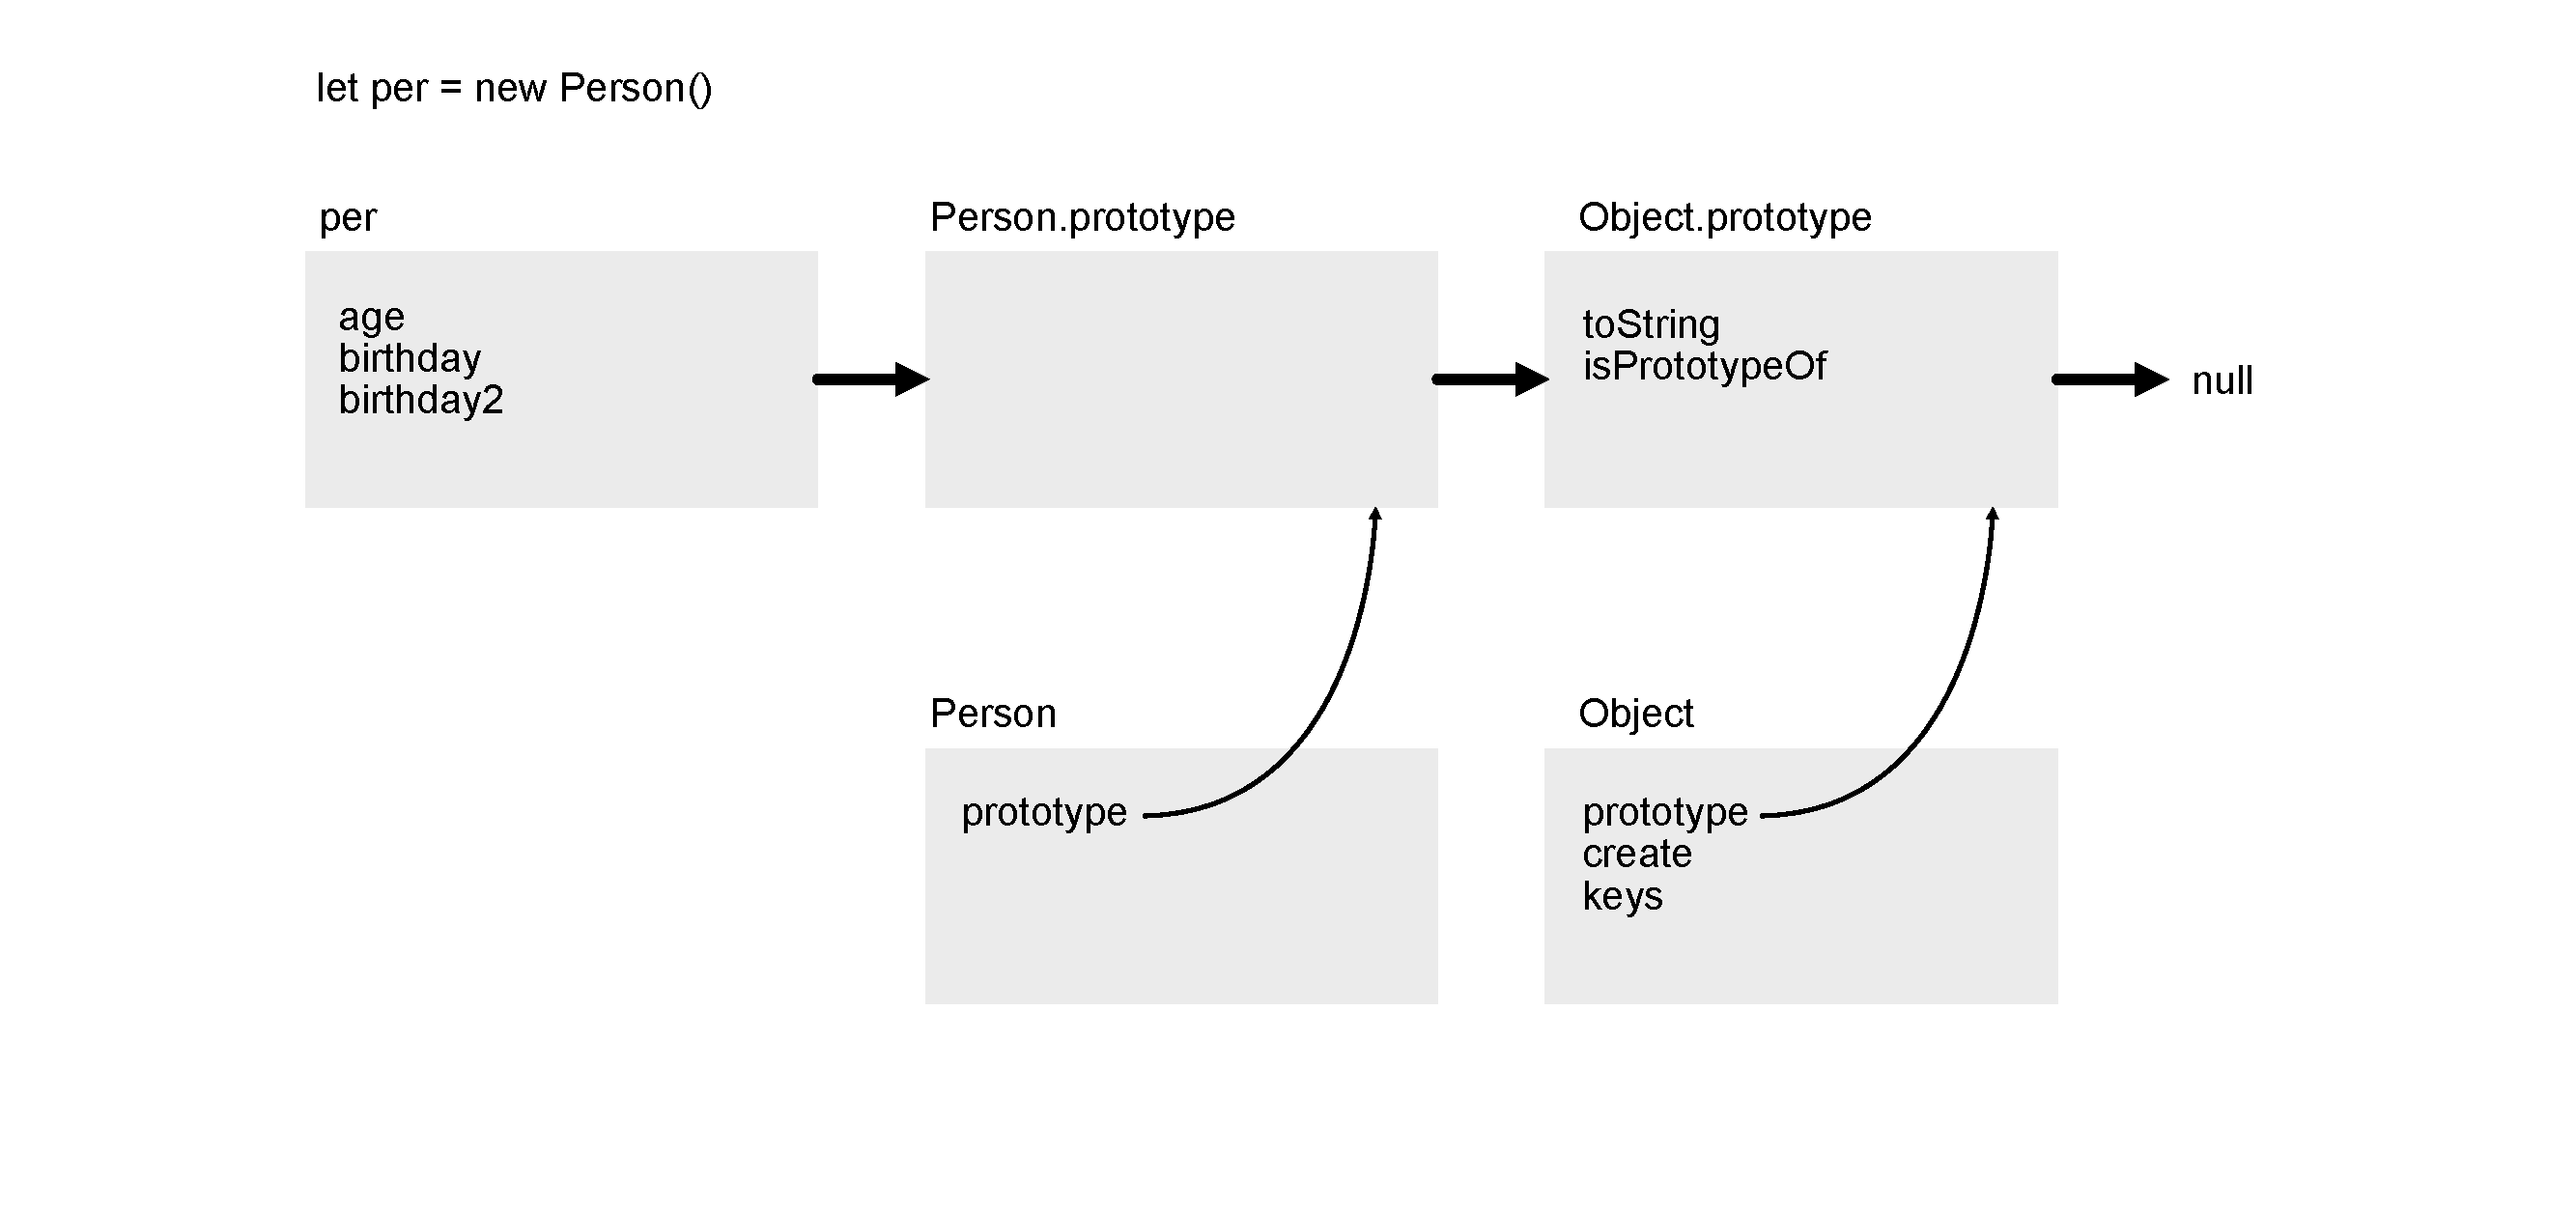
\includegraphics[width=14cm]{img/prototype_chain2}
\end{frame}

%--- Person Example 1 ---------------------------------------------------
\begin{frame}[fragile] \frametitle{prototype}
\begin{CodeBox}{}
function Person() {
  this.age = 0;
}
Person.prototype.birtday = function() { this.age++; };
let per = new Person();
\end{CodeBox}
  \centering
  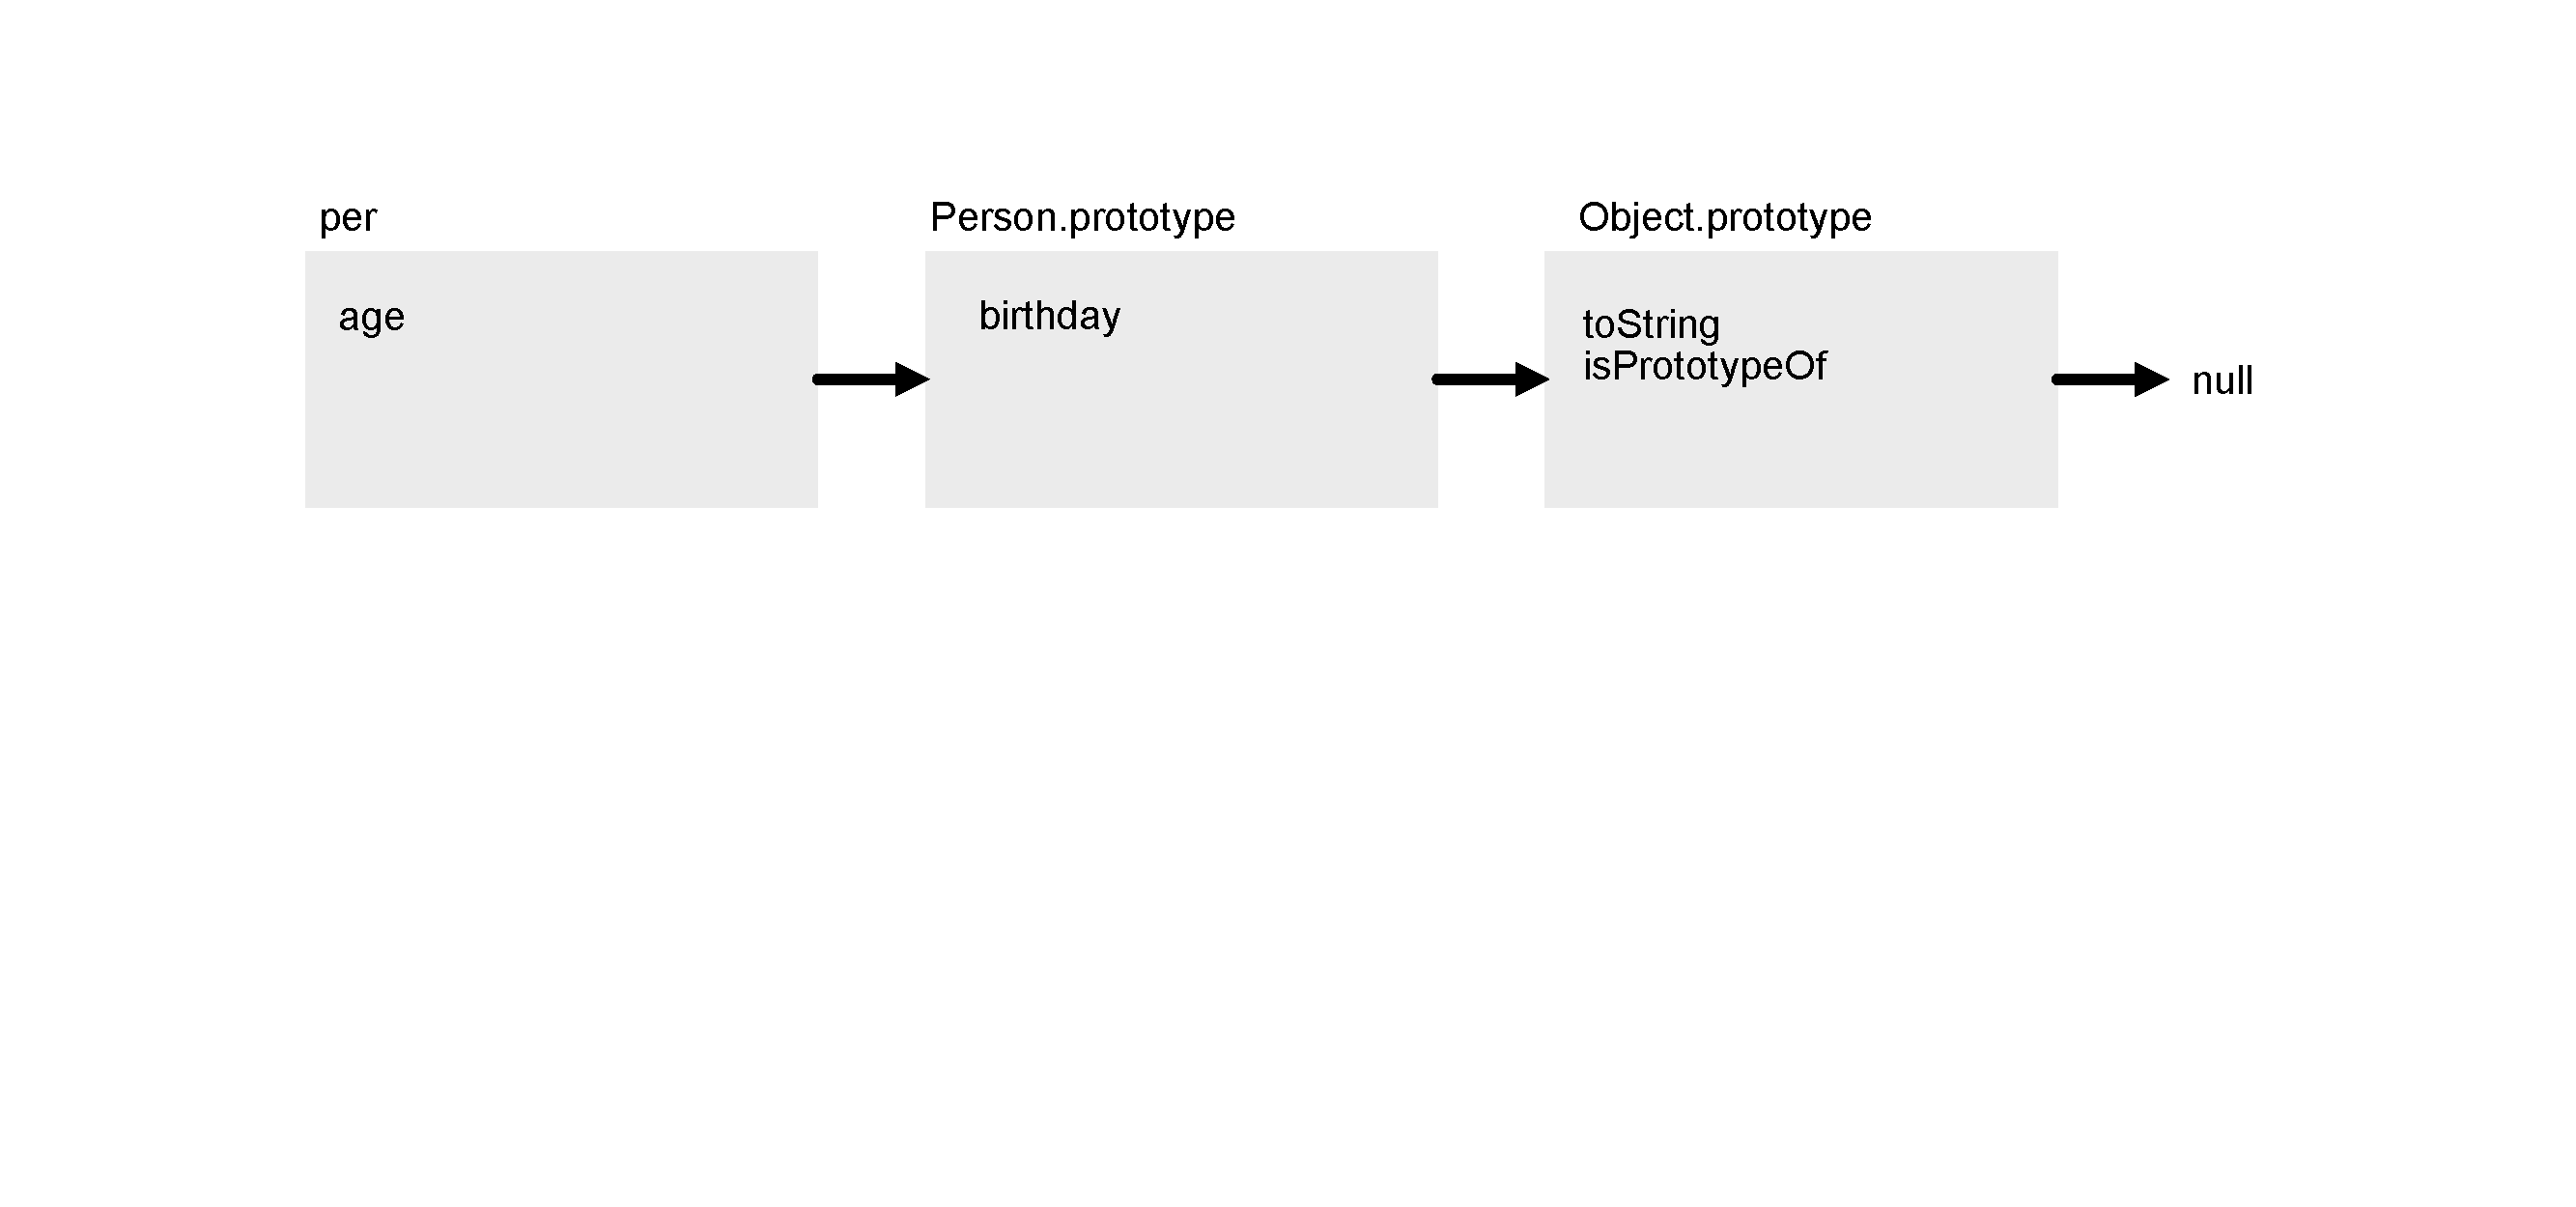
\includegraphics[width=14cm]{img/prototype_chain3}
\end{frame}

%--- Set up Prototype Chain ---------------------------------------------------
\begin{frame}[fragile] \frametitle{Set up Prototype Chain}
Setting up the prototype chain:
\begin{itemize}
  \item \code{new} do the work for you
  \begin{itemize}
    \item all constructor functions have the \code{prototype} property
    \item \code{new}:
    \begin{itemize}
      \item creates an empty object
      \item {\bf and} set its parent in the prototype chain to the \code{prototype} in the constructor function
    \end{itemize}
    \item all properties in the \code{prototype} of the constructor function are now in the prototype chain of the new object
  \end{itemize}
  \item you can do it manually: \code{Object.create()}
\end{itemize}
\end{frame}

%--- Property Name Lookup ---------------------------------------------------
\begin{frame}[fragile] \frametitle{Property Name Lookup}
Property read:
\begin{itemize}
  \item follows the prototype chain
  \item return the first value found
  \item return \code{undefined} if the end of the prototype chain is reached
\end{itemize}
\vspace{8mm}
Property write:
\begin{itemize}
  \item do not follows the prototype chain
  \item writes to the referenced object (left hand side of the dot)
  \item update if the name existed
  \item adds the property if the name did not exist
\end{itemize}
\end{frame}

%--- Person Example 2 ---------------------------------------------------
\begin{frame}[fragile] \frametitle{prototype}
\begin{CodeBox}{}
let cat = new Person();
cat.birtday = function() { this.age += 7; }
\end{CodeBox}
  \centering
  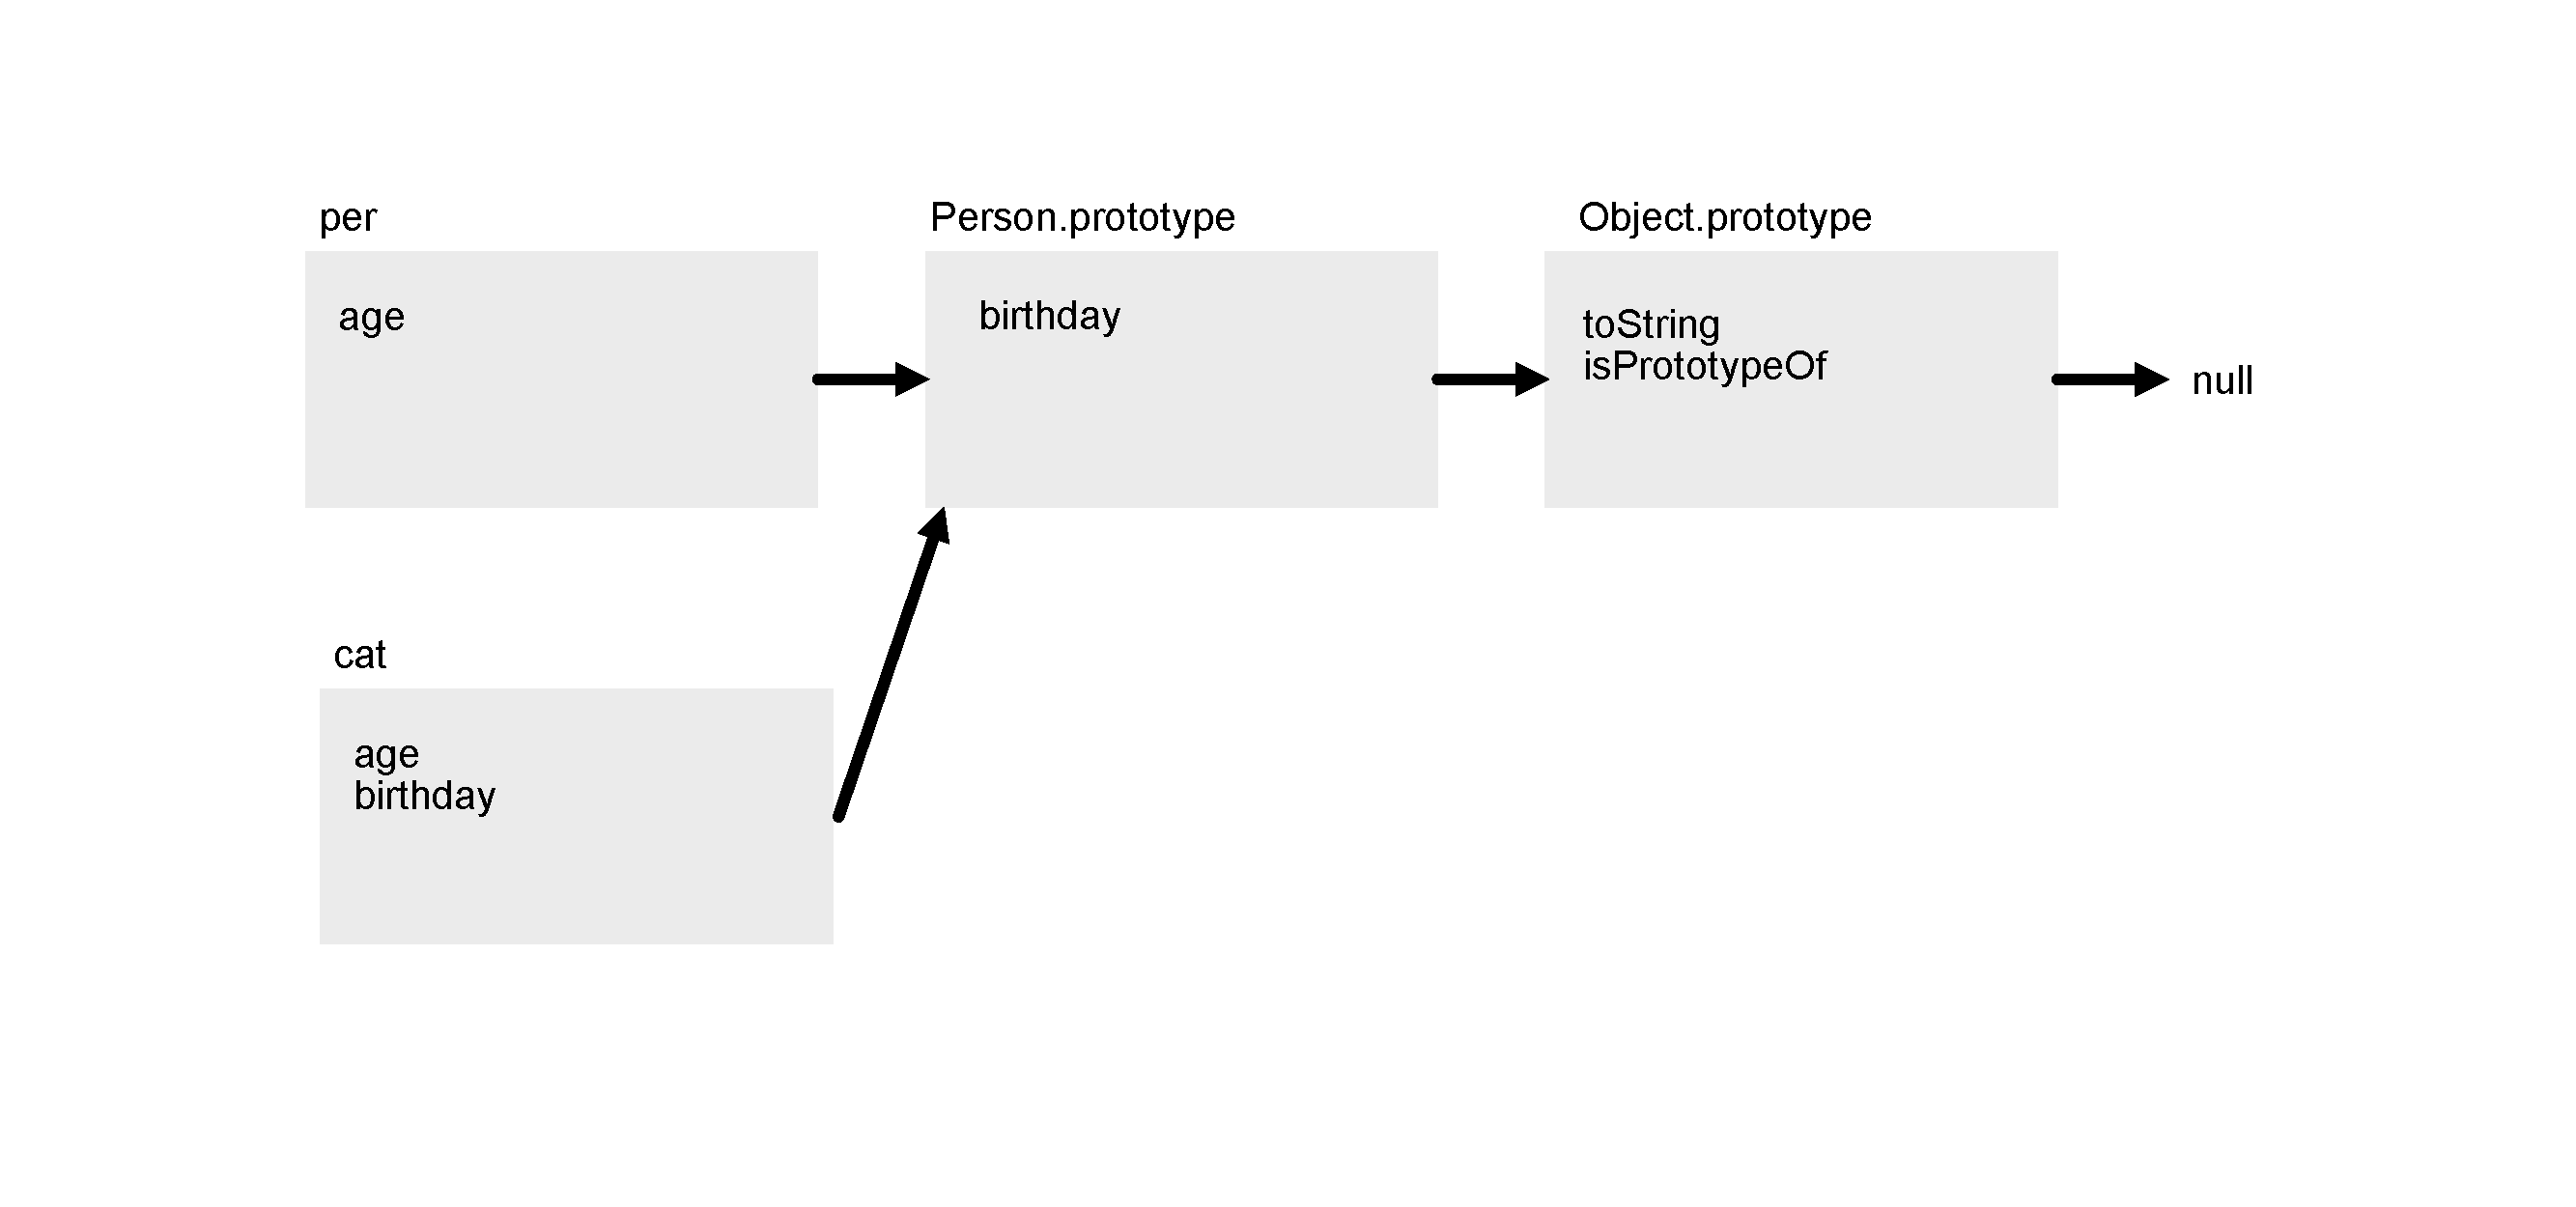
\includegraphics[width=14cm]{img/prototype_chain4}
\end{frame}

%--- Inheritance ---------------------------------------------------
\begin{frame}[fragile] \frametitle{Inheritance}
\begin{itemize}
  \item \code{Object.create()} creates an object with a given prototype chain
  \item store it as the \code{prototype} property in the constructor function
  \item explicit call the constructor of the superclass
\end{itemize}
\vspace{2mm}
\begin{CodeBox}{Cat extends Person}
function Cat() {
  this = Person.call(this);
}
Cat.prototype = Object.create(Person.prototype);
Cat.prototype.birthday = function() { this.age += 7; }
Cat.prototype.toString = function() {
  return 'I am a cat of age ' + this.age';
}
\end{CodeBox}
\end{frame}

%--- Cat Class  ---------------------------------------------------
\begin{frame}[fragile] \frametitle{prototype}
  \centering
  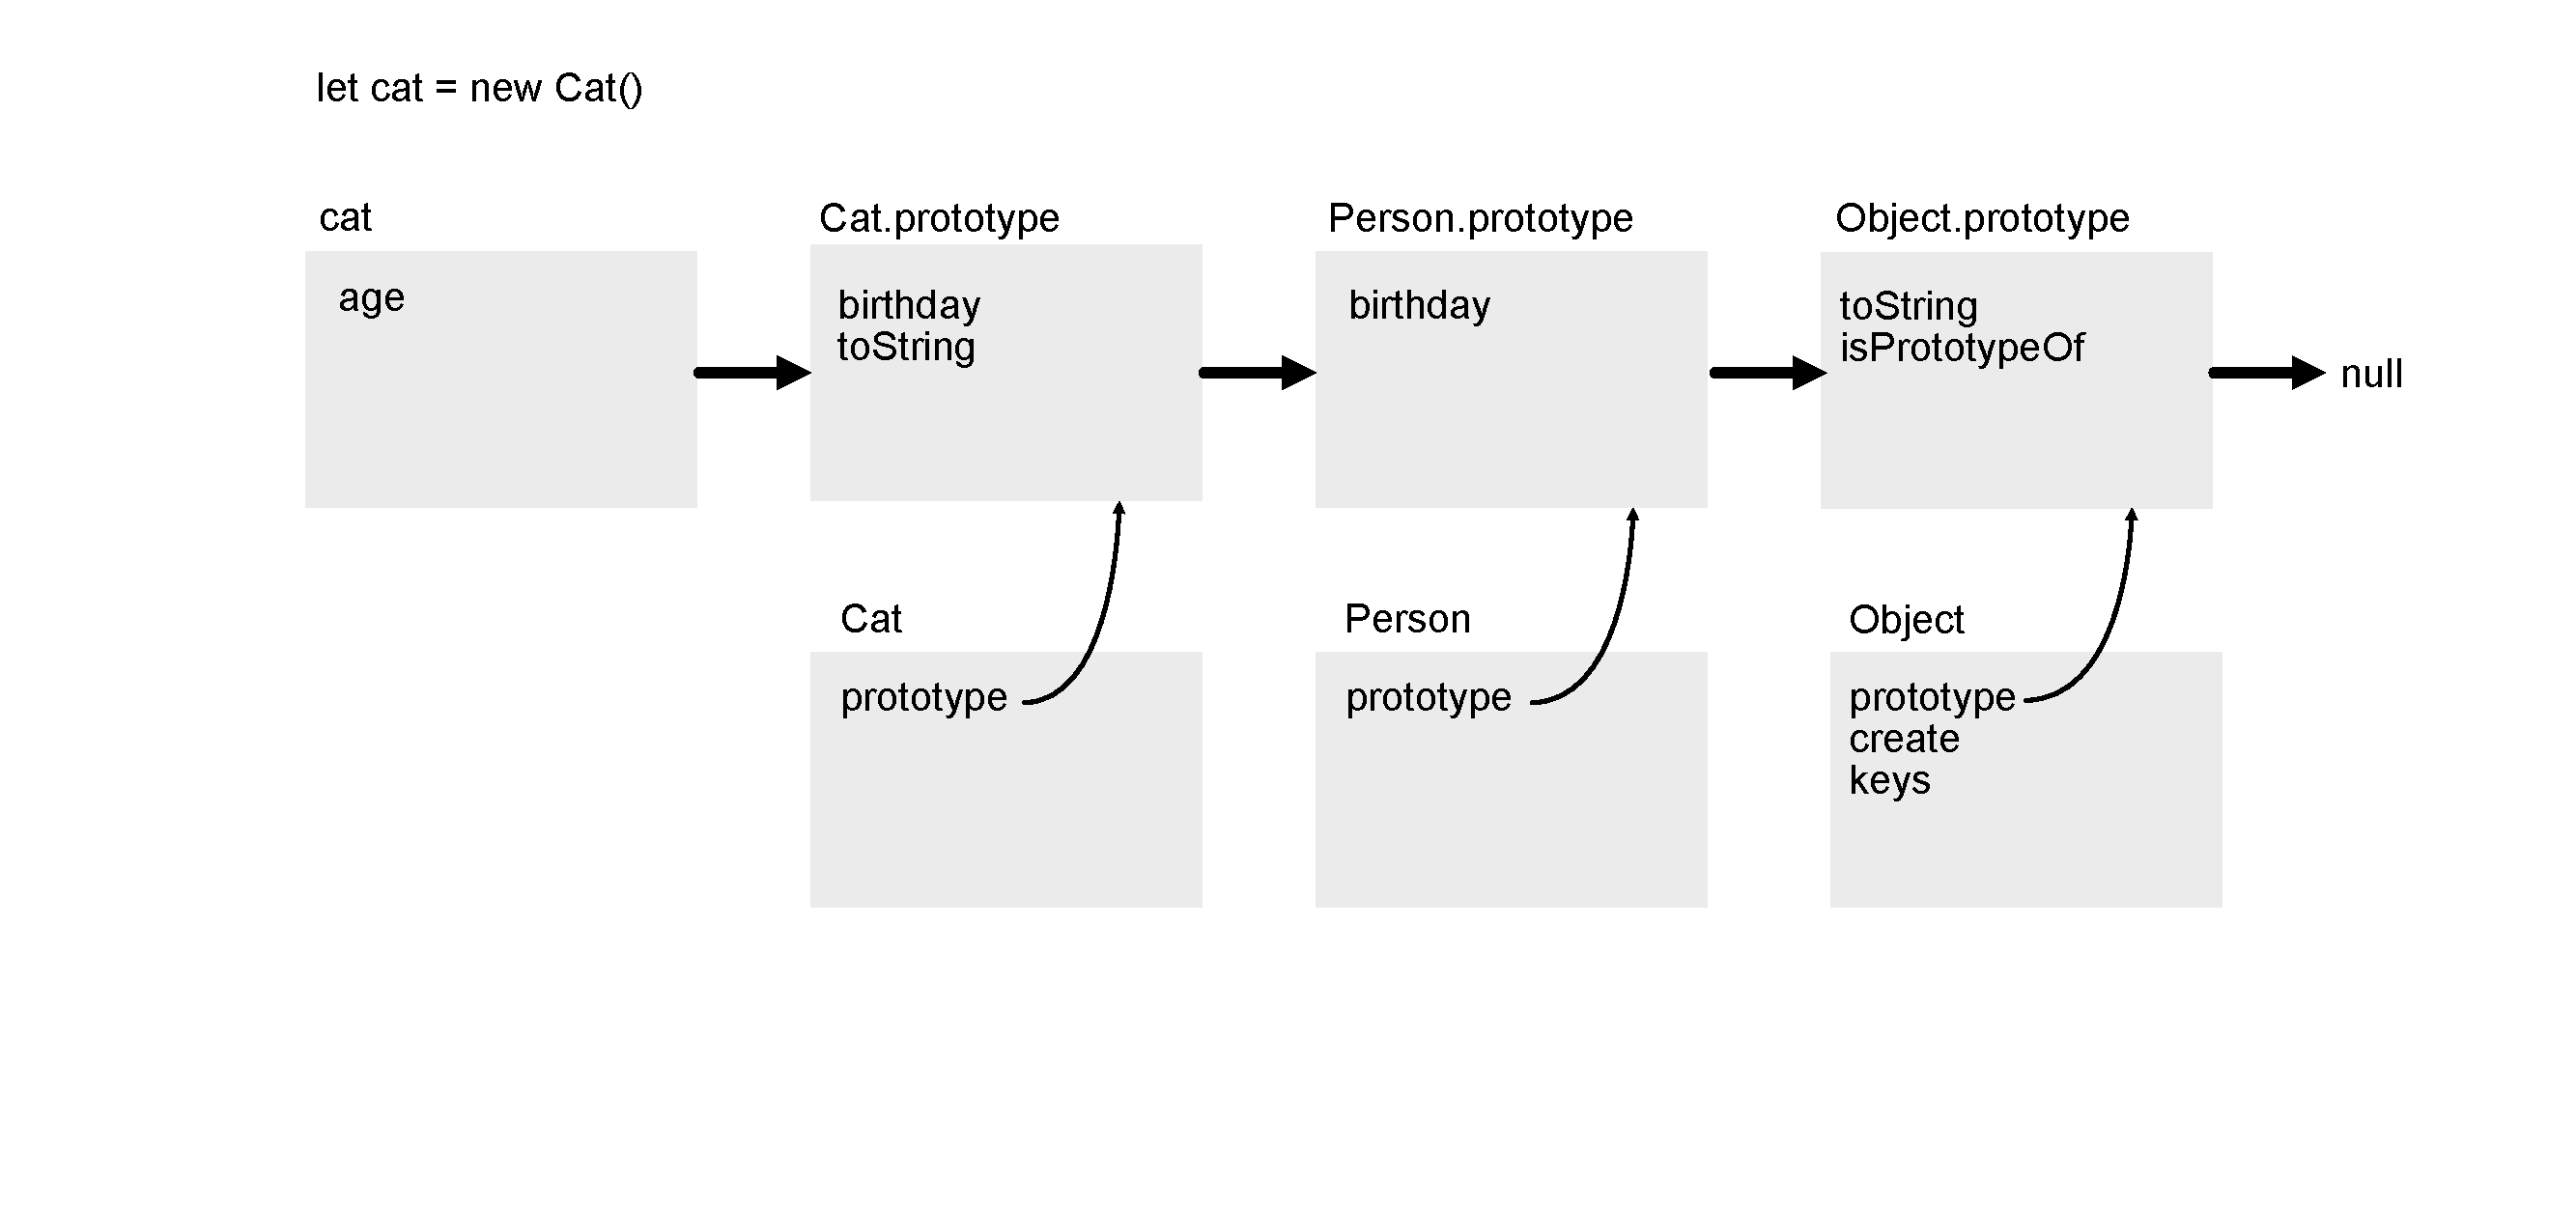
\includegraphics[width=14cm]{img/prototype_chain5}
\end{frame}

%--- Class ---------------------------------------------------
\begin{frame}[fragile] \frametitle{Class}
a "Java class" corresponds to two objects in JavaScript
\begin{itemize}
  \item a constructor function:
  \begin{itemize}
    \item its name is part of the variable name space
    \item place static stuff here
  \end{itemize}
  \item a prototype object
  \begin{itemize}
    \item the object to add to the prototype chain
    \item place any stuff to be inherited by the instances here
  \end{itemize}
\end{itemize}
\vspace{5mm}

\code{Class} was introduced in ECMAScript 2015
\begin{itemize}
  \item syntactical sugar, set up the prototype chin as outlined above
  \item \code{static} will add the property to the constructor function object
  \item \code{public} or \code{#private}
\end{itemize}
\end{frame}
%--- Class Example ---------------------------------------------------
\begin{frame}[fragile] \frametitle{Class Example}
\begin{CodeBox}{}
class Person {
  static #count = 0;

  constructor(age) {
    this.age = age || 0;
    Person.#count = Person.#count + 1;
  }

  birthday() {
    this.age++;
  }
}
\end{CodeBox}
\end{frame}

%--- Class Picture  ---------------------------------------------------
\begin{frame}[fragile] \frametitle{prototype}
  \centering
  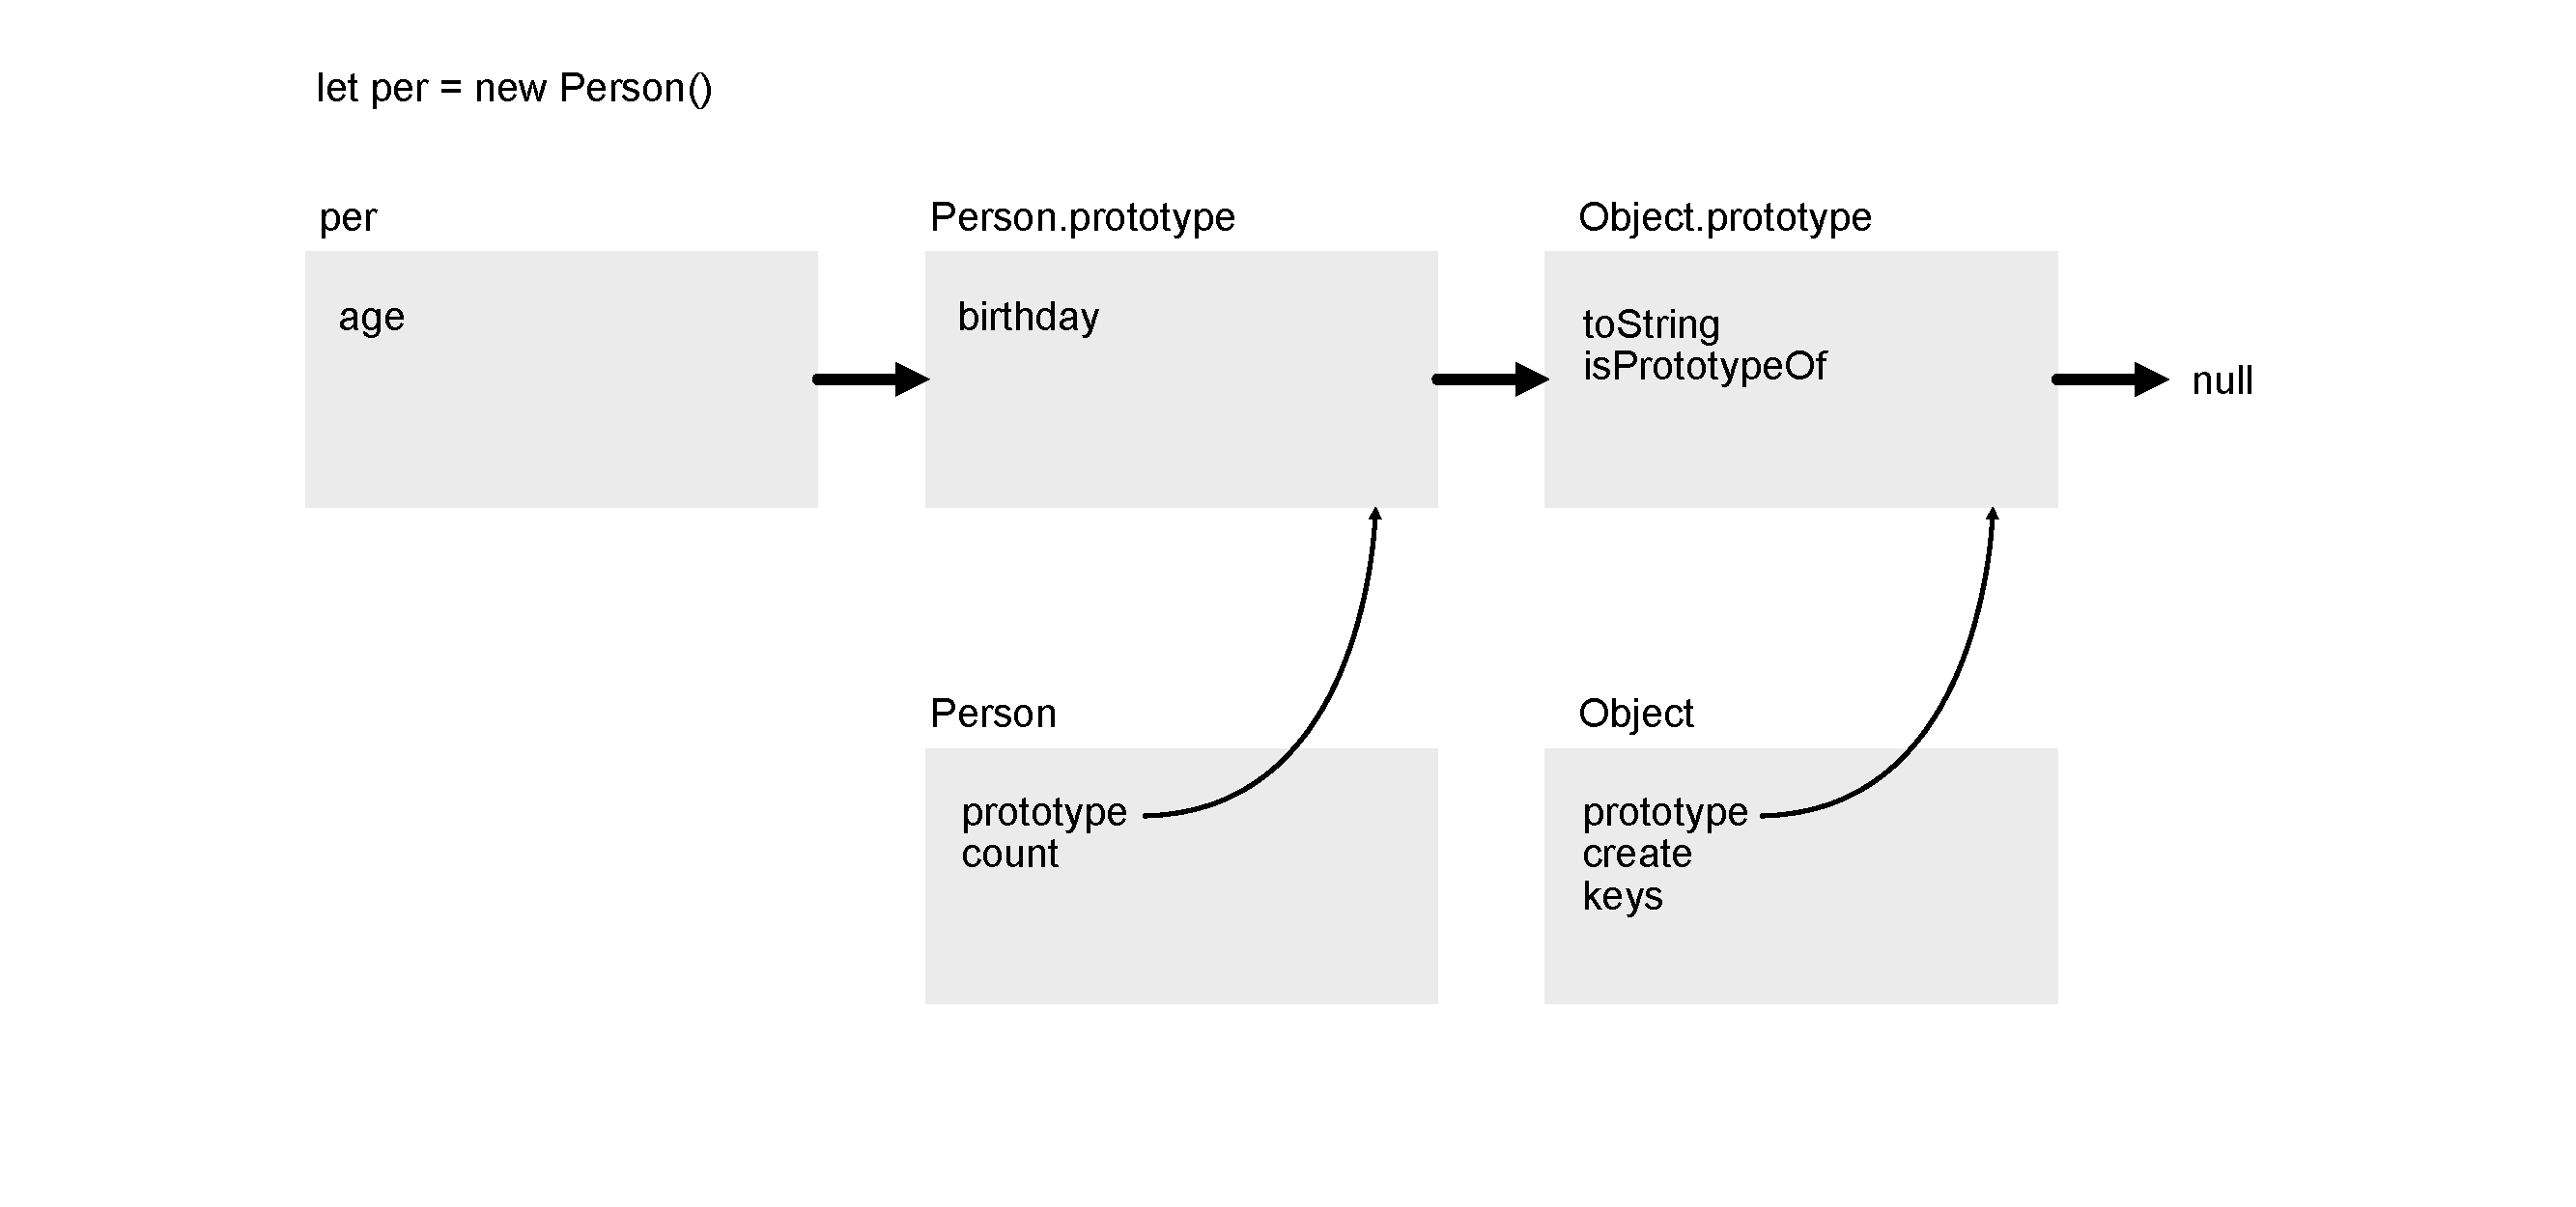
\includegraphics[width=14cm]{img/prototype_chain6}
\end{frame}


%--- Class Extends---------------------------------------------------
\begin{frame}[fragile] \frametitle{Class Extends}
The constructor:
\begin{itemize}
  \item in a derived class must call \code{super()} before you can access \code{this}
  \item in a base class may not call \code{super()}
\end{itemize}
\begin{CodeBox}{}
class Cat extends Person {
  constructor(age) {
    super(age);
  }
  birthday() {
    this.age += 7;
  }
  toString() {
    return 'I am a cat of age ' + this.age';
  }
}
\end{CodeBox}
\end{frame}

%---Undefined Names ---------------------------------------------------
\begin{frame}[fragile] \frametitle{Access to Undefined Names}
Variables and properties have distinct name spaces.
\\ \vspace{4mm}
Name Scope: Variables and Parameters
\begin{itemize}
  \item read: throws ReferenceError
  \item write: creates a variable in the global scope
\end{itemize}
\vspace{5mm}
Objects: Properties
\begin{itemize}
  \item read: evaluates to \code{undefined}
  \item write: adds the property to the object
\end{itemize}
\end{frame}

%--- Standard Classes---------------------------------------------------
\begin{frame}[fragile] \frametitle{Standard Classes}
In JavaScript there are many standard classes. Some important: 
\begin{itemize}
  \item \code{Object} - default base class for all objects
  \item \code{Function extends Object} - base class for all functions
  \item \code{Array} - base class for array litterals
\end{itemize}
\end{frame}

%--- Property Properties---------------------------------------------------
\begin{frame}[fragile] \frametitle{Property Descriptors}
Distinction between
\begin{itemize}
  \item \emph{own properties}
  \item \emph{inherited properties}
\end{itemize}

Object properties have descriptors (metadata)
\begin{itemize}
  \item \emph{value}
  \item \emph{writable}
  \item \emph{configurable}
  \item \emph{enumerable}
\end{itemize}
\end{frame}

%--- Iteration---------------------------------------------------
\begin{frame}[fragile] \frametitle{Iteration}
Iterating over object property names and values
\begin{itemize}
  \item \code{for ... in} --- all enumerable string properties (include inherited)
  \item \code{Object.keys()} --- own enumerable
  \item \code{Object.values()} --- own enumerable
  \item \code{Object.entries()} --- own enumerable
  \item \code{Object.getOwnPropertyNames()} --- own
  \item \code{...}, spread --- own enumerable
\end{itemize}
\end{frame}

%--- More to learn---------------------------------------------------
\begin{frame}[fragile] \frametitle{More to learn}

The JavaScript syntax only give you access to a subset of the language\ldots
\vspace{8mm}
\begin{CodeBox}{}
Object.defineProperty(obj, "prop", {
    value: "test",
    writable: false
});
\end{CodeBox}
\vspace{8mm}
This is however out of scope for this course.
\end{frame}

